%\documentclass[gray,handout, pdftex, 11pt]{beamer}
%\documentclass[handout, pdftex, 11pt]{beamer}
\documentclass[pdftex, 11pt]{beamer}

\usepackage{pgfpages}
\usepackage[utf8]{inputenc}
\usepackage[T1]{fontenc}
\usepackage{lmodern}
%\usepackage[italian]{babel}
\usepackage{graphicx}
\usepackage{microtype}
\usepackage{acronym}
\usepackage{array}
%\usepackage{natbib}

\usepackage{tikz}
\usetikzlibrary{intersections, arrows, shapes, decorations.pathreplacing, decorations.pathmorphing, calc}

\usepackage{appendixnumberbeamer}

\mode<presentation>{
  %-------------------------1
  \usetheme{Boadilla}
  \usecolortheme{beaver}
  %-------------------------1
  %-------------------------2
  %\usetheme{Goettingen}
  %\usecolortheme{sidebartab}
  %-------------------------2
  %\useoutertheme[right]{sidebar}
  %\usefonttheme{default}
  \setbeamercovered{transparent}
  %\setbeameroption{show notes on second screen=right}
  \setbeamertemplate{navigation symbols}{}

  \bibliographystyle{abbrv}  
  %\renewcommand\bibfont{\scriptsize}
  \setbeamertemplate{bibliography item}{\textbullet}
  \setbeamertemplate{itemize item}{\checkmark}
  \setbeamertemplate{itemize subitem}{-}
  \setbeamertemplate{enumerate items}[default]
  \setbeamertemplate{sections/subsections in toc}[square]
}

%stili
\tikzstyle{linea}=[draw, green]
\tikzstyle{service}=[very thick, draw, blue]
\tikzstyle{newService}=[very thick, draw, red]
\tikzstyle{modulo}=[thick, draw, black]
\tikzstyle{freccia}=[->, very thick, >=stealth', draw, red]


\newcommand{\frecciadx}{~{\tikz[baseline] \draw[freccia] (0,0.5ex) --
  (5.5ex,0.5ex);}~}

\title[Test status]{\textbf{Test status}}
\subtitle{tkLayout developers meeting}
\institute[CERN]{
  %{\Large\textbf{CERN}}\\{European Organization for Nuclear Research}\\[0.5cm]
  %\\[0.2cm]
  European Organization for Nuclear Research\\[0.5cm]
  
\includegraphics[width=2cm]{img/LogoBadge.pdf}\\
}

\author[Stefano Martina]{
  %\\[0.2cm]
  \textbf{Stefano MARTINA}\\
  {\small stefano.martina@cern.ch}
}

\date[\today]{\flushright \today}

\begin{document}

\begin{frame}[plain,noframenumbering]
  \titlepage
\end{frame}

\begin{frame}{Testing algorithm}
  \begin{enumerate}
  \item Build test case with controlled amount of material
  \item Get elements \alert{coordinates}
    \begin{itemize}
    \item [$\to$] from tklayout run
    \end{itemize}
  \item Build model with \alert{expected} material in each element
  \item Identify \alert{areas} in $\eta$ with same effect
    \begin{itemize}
    \item[$\to$] where same object are superimposed in $\eta$
    \end{itemize}
  \item \alert{Calculate} weight in radiation length
  \item \alert{Correlate} tklayout \alert{output} with \alert{expected} calculation
  \end{enumerate}
\end{frame}

\begin{frame}{Compute expected material for \emph{g/m} unit}
  \begin{block}{Cylinder, \alert{$L$} $g/mm$ of material \alert{M}}
    $$
    \frac{X_0}{X_{0M}} = \frac{L}{2\pi r \cdot X_{0M}} \cdot \frac{e^\eta+e^{-\eta}}{2}
    $$
  \end{block}
  \begin{block}{Disk, \alert{L} $g/mm$ of material \alert{M}}
    $$
    \frac{X_0}{X_{0M}} = \frac{L}{\pi(r_1+r_2)\cdot X_{0M}}\cdot\frac{e^{2\eta}+1}{e^{2\eta}-1}
    $$
  \end{block}

  \begin{itemize}
  \item For \alert{layers} rods, \alert{$L$} is:
    \begin{itemize}
    \item [$\to$] the set material multiplied by the number of rods
    \end{itemize}
  \item For \alert{disks} ``rods'', \alert{$L$} is:
    \begin{itemize}
    \item [$\to$] the set material multiplied by the number of modules of the first ring
    \end{itemize}
  \end{itemize}
\end{frame}

\begin{frame}{Compute expected material for \emph{mm} unit}
  \begin{block}{Cylinder, \alert{$L$} $mm$ of material \alert{M}}
    $$
    \frac{X_0}{X_{0M}} = \frac{L\cdot\rho_M}{X_{0M}}\cdot\frac{e^\eta+e^{-\eta}}{2}
    $$
  \end{block}
  \begin{block}{Disk, \alert{$L$} $mm$ of material \alert{M}}
    $$
    \frac{X_0}{X_{0M}} = \frac{L\cdot\rho_M}{X_{0M}}\cdot\frac{e^{2\eta}+1}{e^{2\eta}-1}
    $$
  \end{block}

  \begin{itemize}
  \item For \alert{layers} and \alert{disks} rods, \alert{$L$} is:
    \begin{itemize}
    \item[$\to$] the set material (not replicated for rod or modules)
    \end{itemize}
  \item[!] \alert{new discovered bug, corrected but still need to rerun tests}
    \begin{itemize}
    \item before, each mm definition where replicated by rods
    \end{itemize}
  \end{itemize}
\end{frame}

\begin{frame}{Compute expected material for \emph{g} unit}
  \begin{block}{Cylinder, \alert{$L$} $g$ of material \alert{M}}
    $$
    \frac{X_0}{X_{0M}} = \frac{L}{2\pi r (z_2-z_1) \cdot X_{0M}} \cdot \frac{e^\eta+e^{-\eta}}{2}
    $$
  \end{block}
  \begin{block}{Disk, \alert{L} $g$ of material \alert{M}}
    $$
    \frac{X_0}{X_{0M}} = \frac{L}{\pi(r_2^2-r_1^2)\cdot X_{0M}}\cdot\frac{e^{2\eta}+1}{e^{2\eta}-1}
    $$
  \end{block}
  \begin{itemize}
  \item Unit \alert{g} can't be used for rods in layers and disks
  \end{itemize}
\end{frame}

\begin{frame}
  \begin{block}{Test1a}
    \alert{$100 g/m$} of \emph{Cu} in the rods of the first layer of the pixel barrel
    \begin{itemize}
    \item \alert{12} rods
    \item \alert{$L=1200$} for every element
    \end{itemize}
  \end{block}
  \begin{center}
    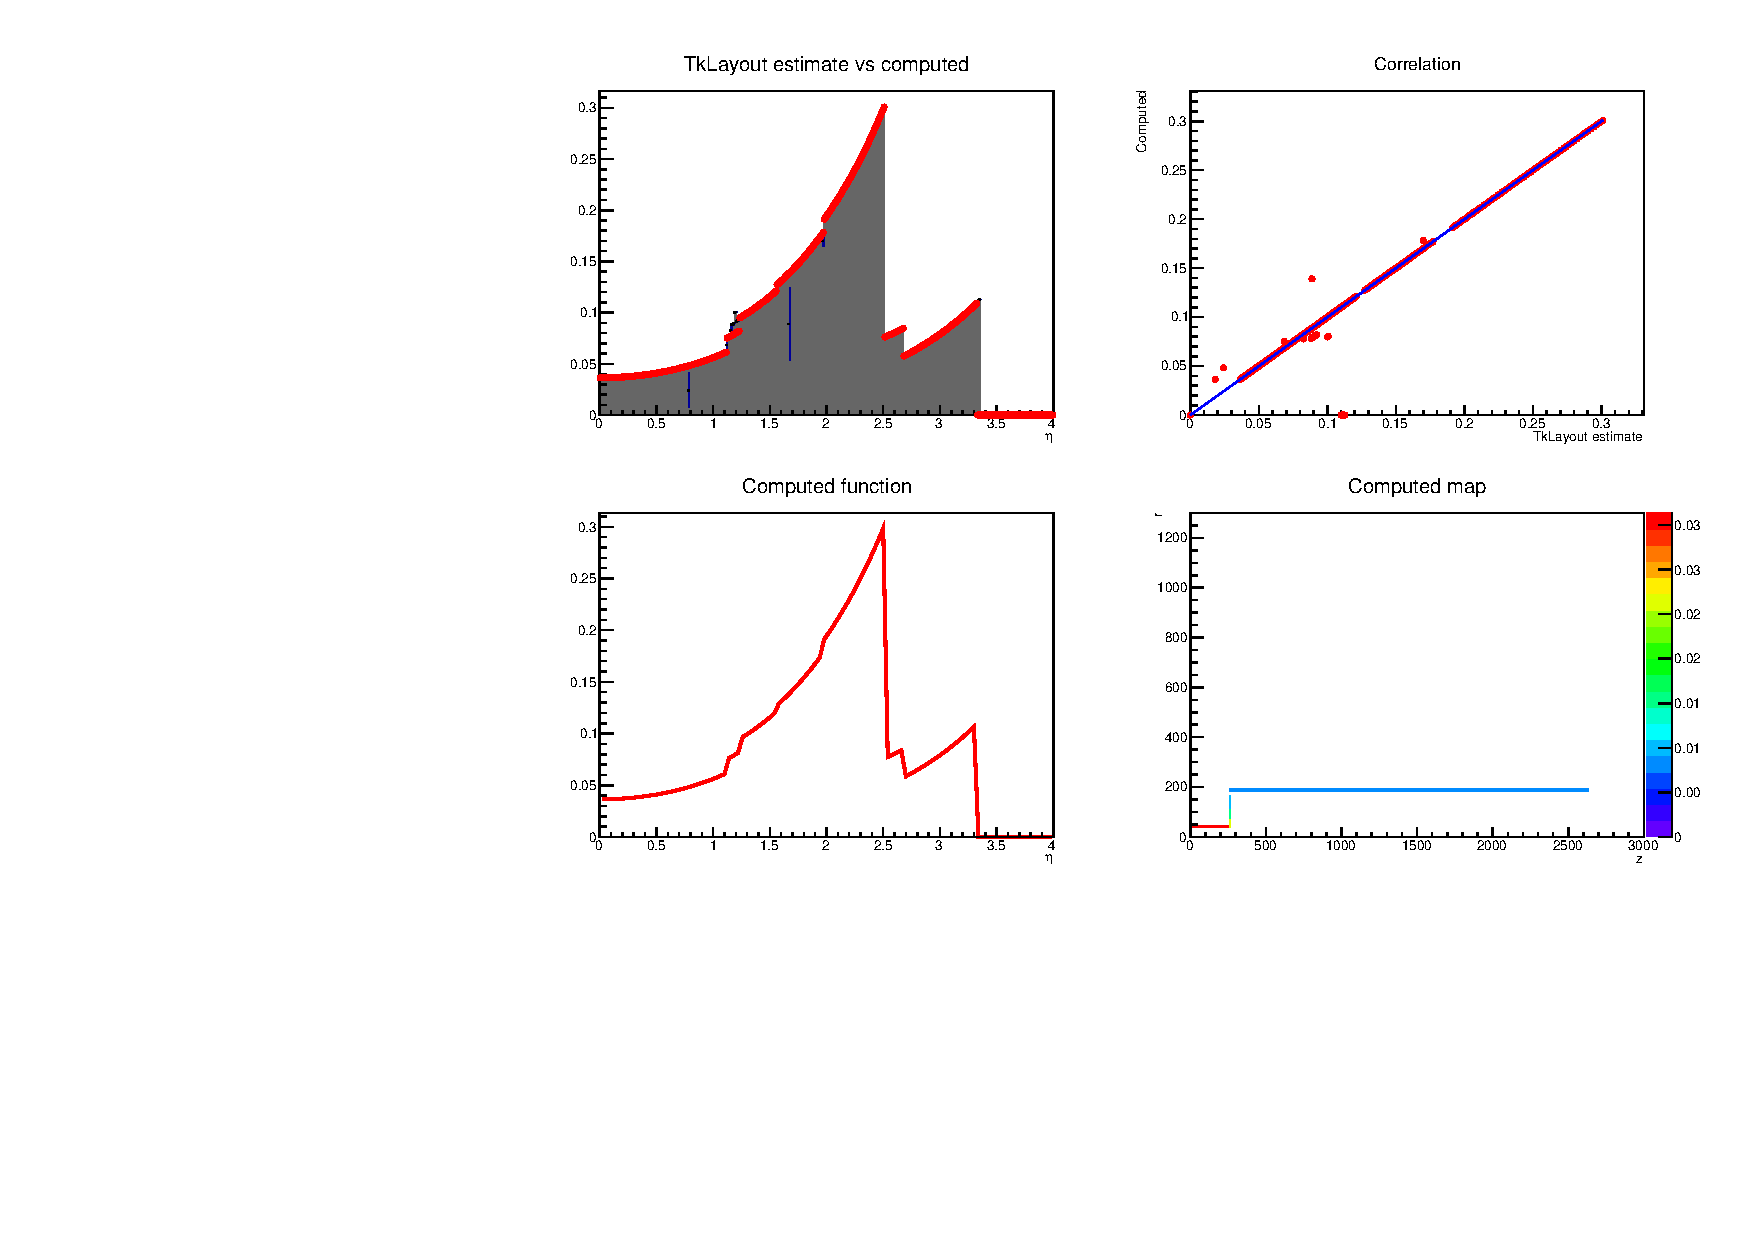
\includegraphics[width=9cm]{img/test1a.pdf}
  \end{center}
\end{frame}

\begin{frame}
  \begin{block}{Test1b}
    \alert{$100 g/m$} of \emph{Cu}  in the rods of the second layer of the pixel barrel
    \begin{itemize}
    \item \alert{24} rods
    \item \alert{$L=2400$} for every element
    \end{itemize}
  \end{block}
  \begin{center}
    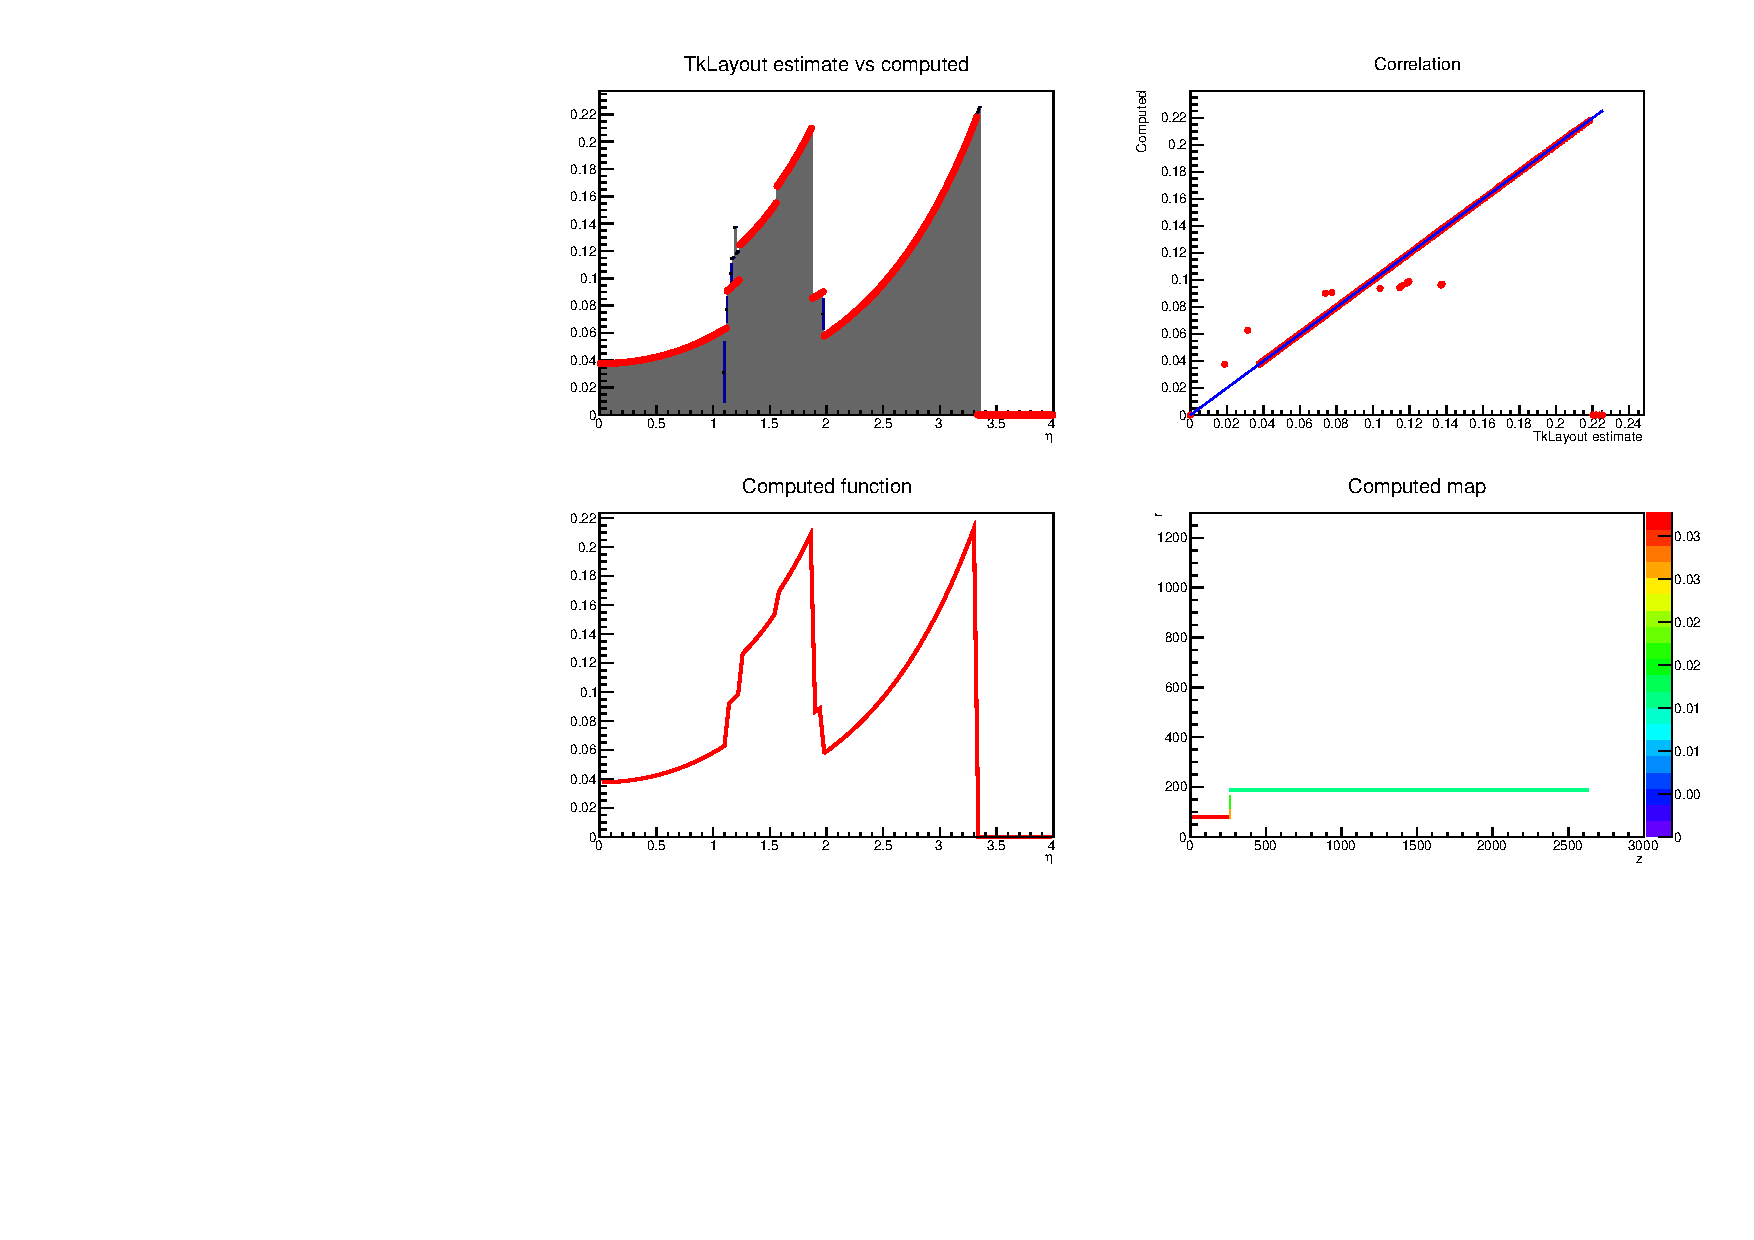
\includegraphics[width=9cm]{img/test1b.pdf}
  \end{center}
\end{frame}

\begin{frame}
  \begin{block}{Test1c}
    \alert{$100 g/m$} of \emph{Cu}  in the rods of the third layer of the pixel barrel
    \begin{itemize}
    \item \alert{36} rods
    \item \alert{$L=3600$} for every element
    \end{itemize}
  \end{block}
  \begin{center}
    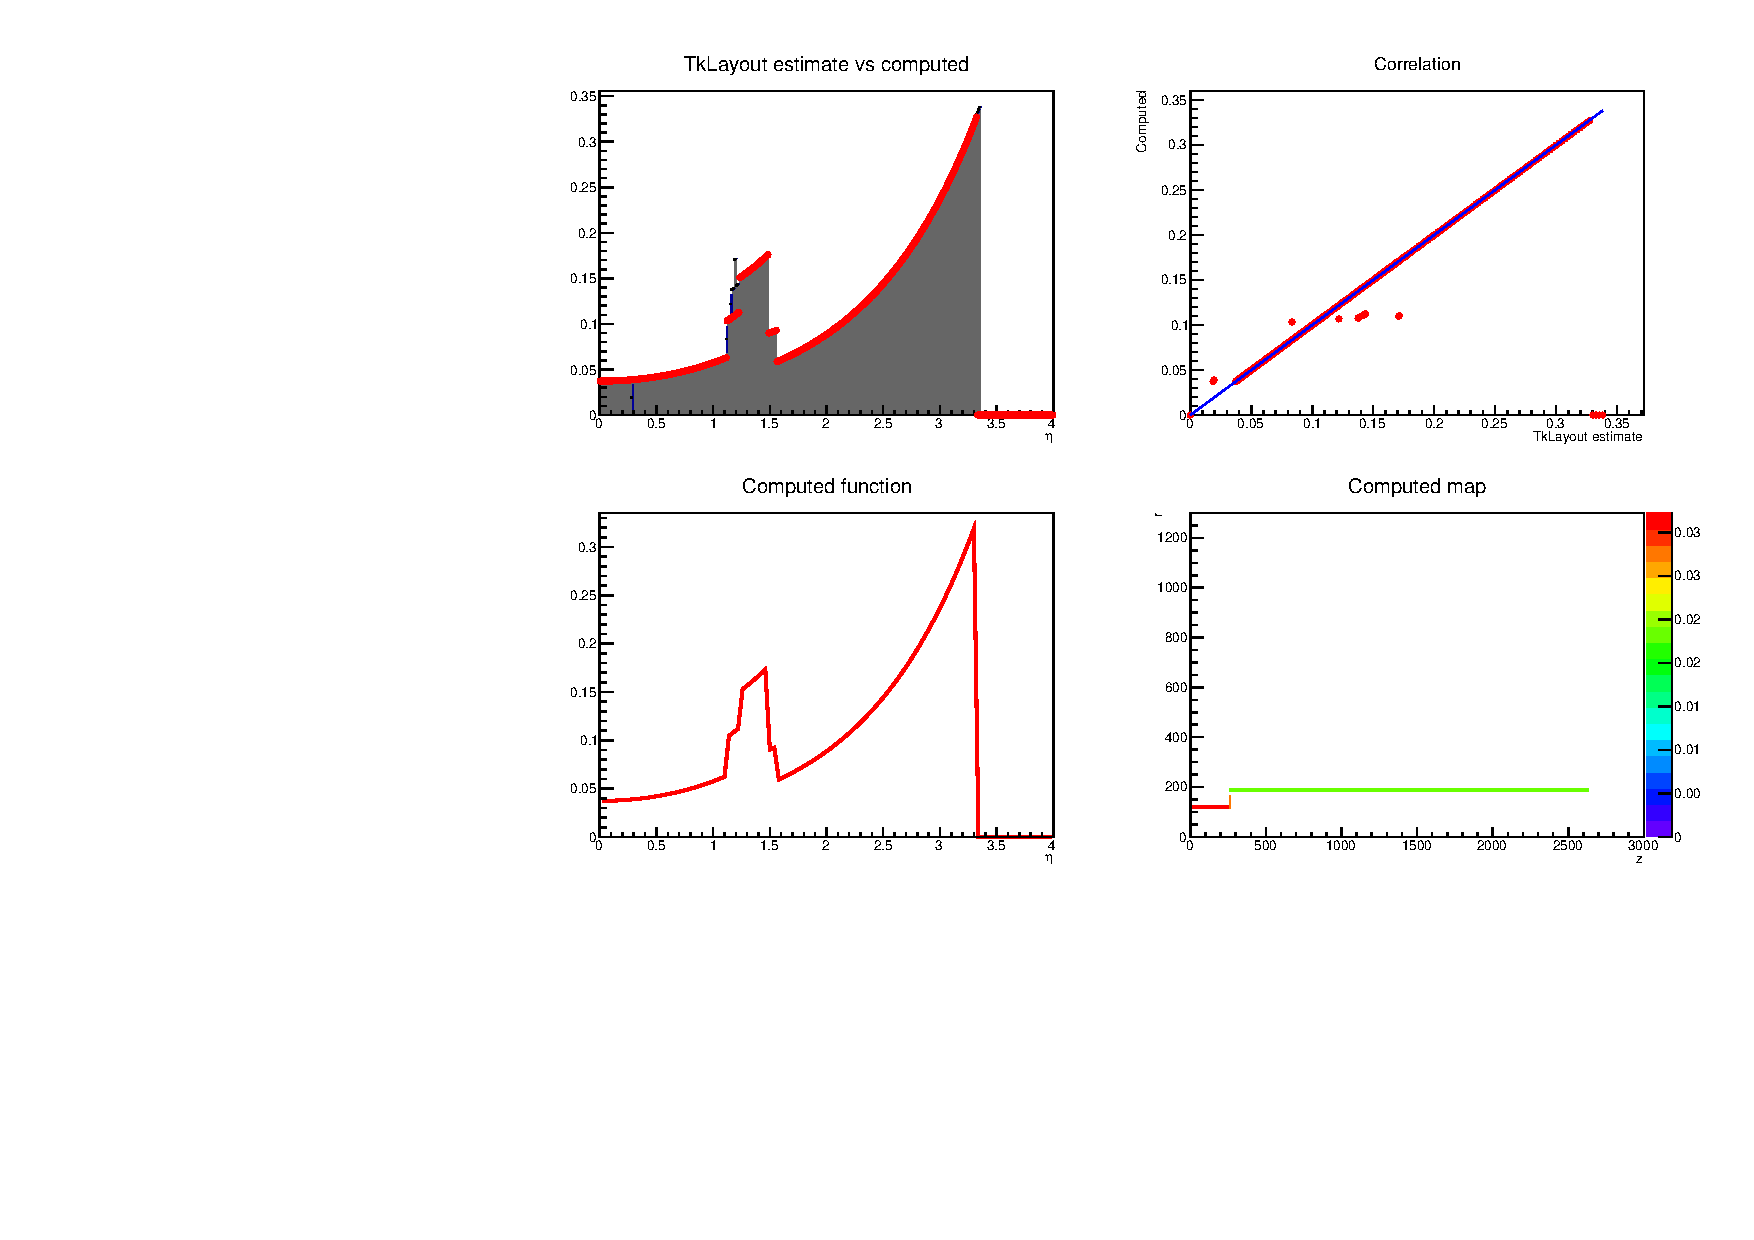
\includegraphics[width=9cm]{img/test1c.pdf}
  \end{center}
\end{frame}

\begin{frame}
  \begin{block}{Test1d}
    \alert{$100 g/m$} of \emph{Cu}  in the rods of the fourth layer of the pixel barrel
    \begin{itemize}
    \item \alert{52} rods
    \item \alert{$L=5200$} for every element
    \end{itemize}
  \end{block}
  \begin{center}
    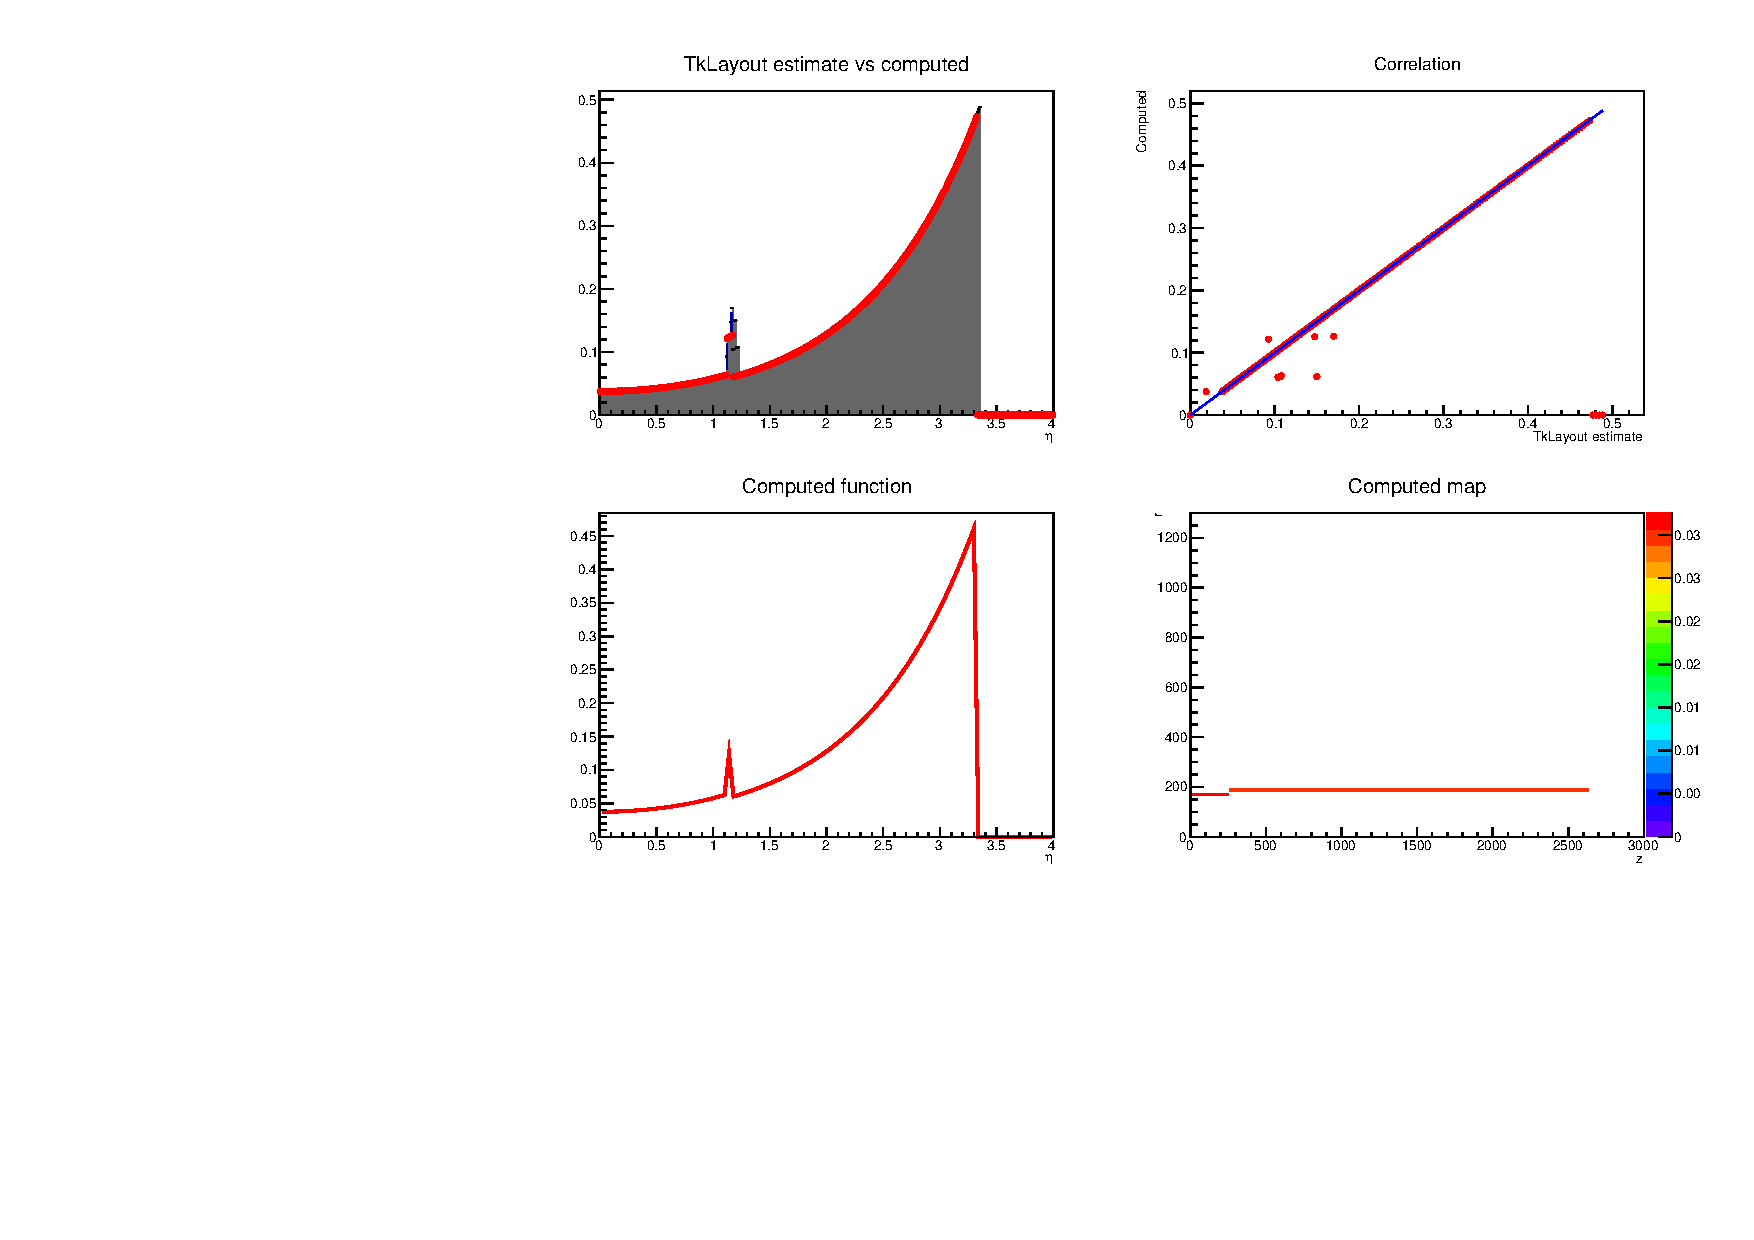
\includegraphics[width=9cm]{img/test1d.pdf}
  \end{center}
\end{frame}

\begin{frame}
  \begin{block}{Test2}
    \alert{$100 g/m$} of \emph{Cu}  in the rods of all the layers of the pixel barrel
    \begin{itemize}
    \item \alert{$L=rods*100$} for layers
    \item \alert{$L=L_{attached layer}+L_{attached disk}$} for disks and last cylinder
    \end{itemize}
  \end{block}
  \begin{center}
    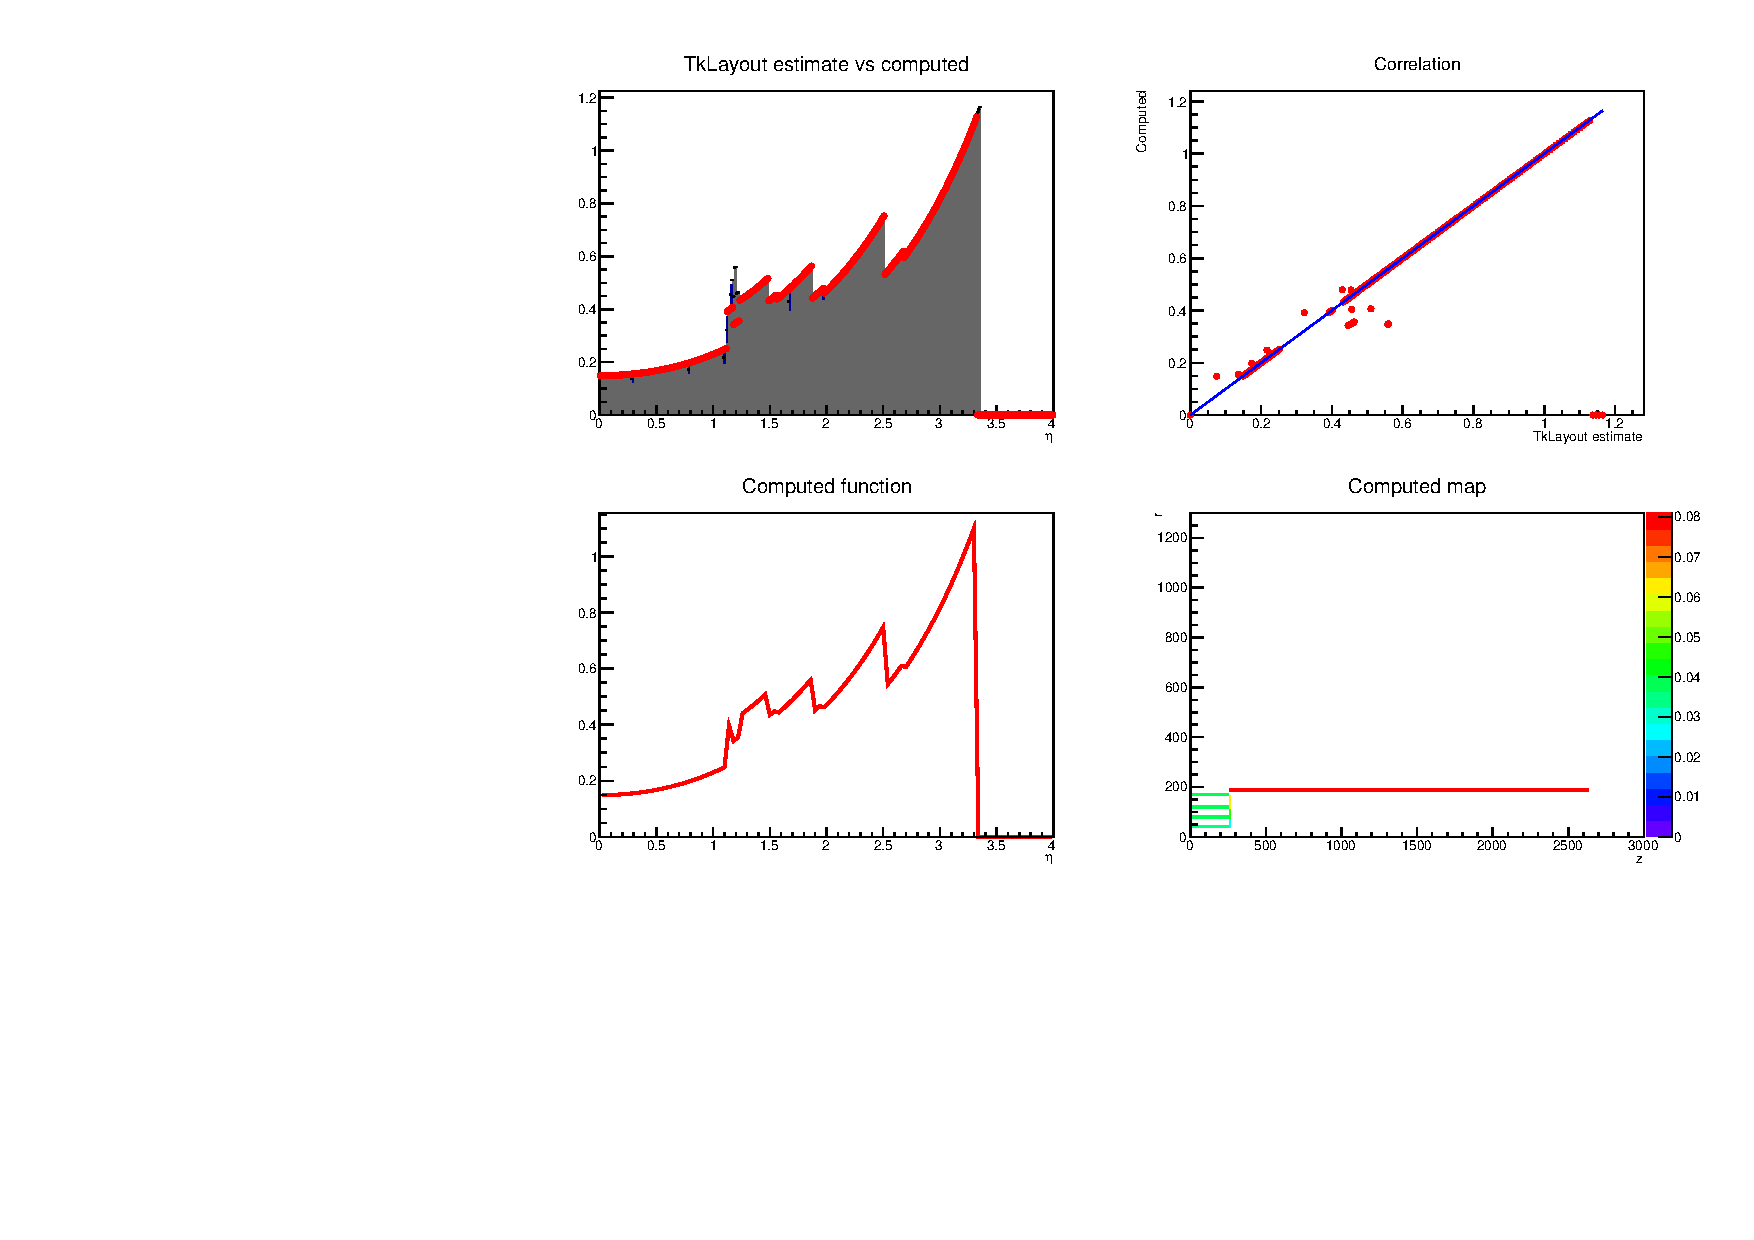
\includegraphics[width=9cm]{img/test2.pdf}
  \end{center}
\end{frame}

\begin{frame}
  \begin{block}{Test3  \alert{WILL CHANGE WITH BUGFIX}}
    \alert{$0.1 mm$} of \emph{Cu}  in the rods of all the layers of the pixel barrel
    \begin{itemize}
    \item \alert{$L=rods*0.1$} for layers
    \item \alert{$L=L_{attached layer}+L_{attached disk}$} for disks and last cylinder
    \end{itemize}
  \end{block}
  \begin{center}
    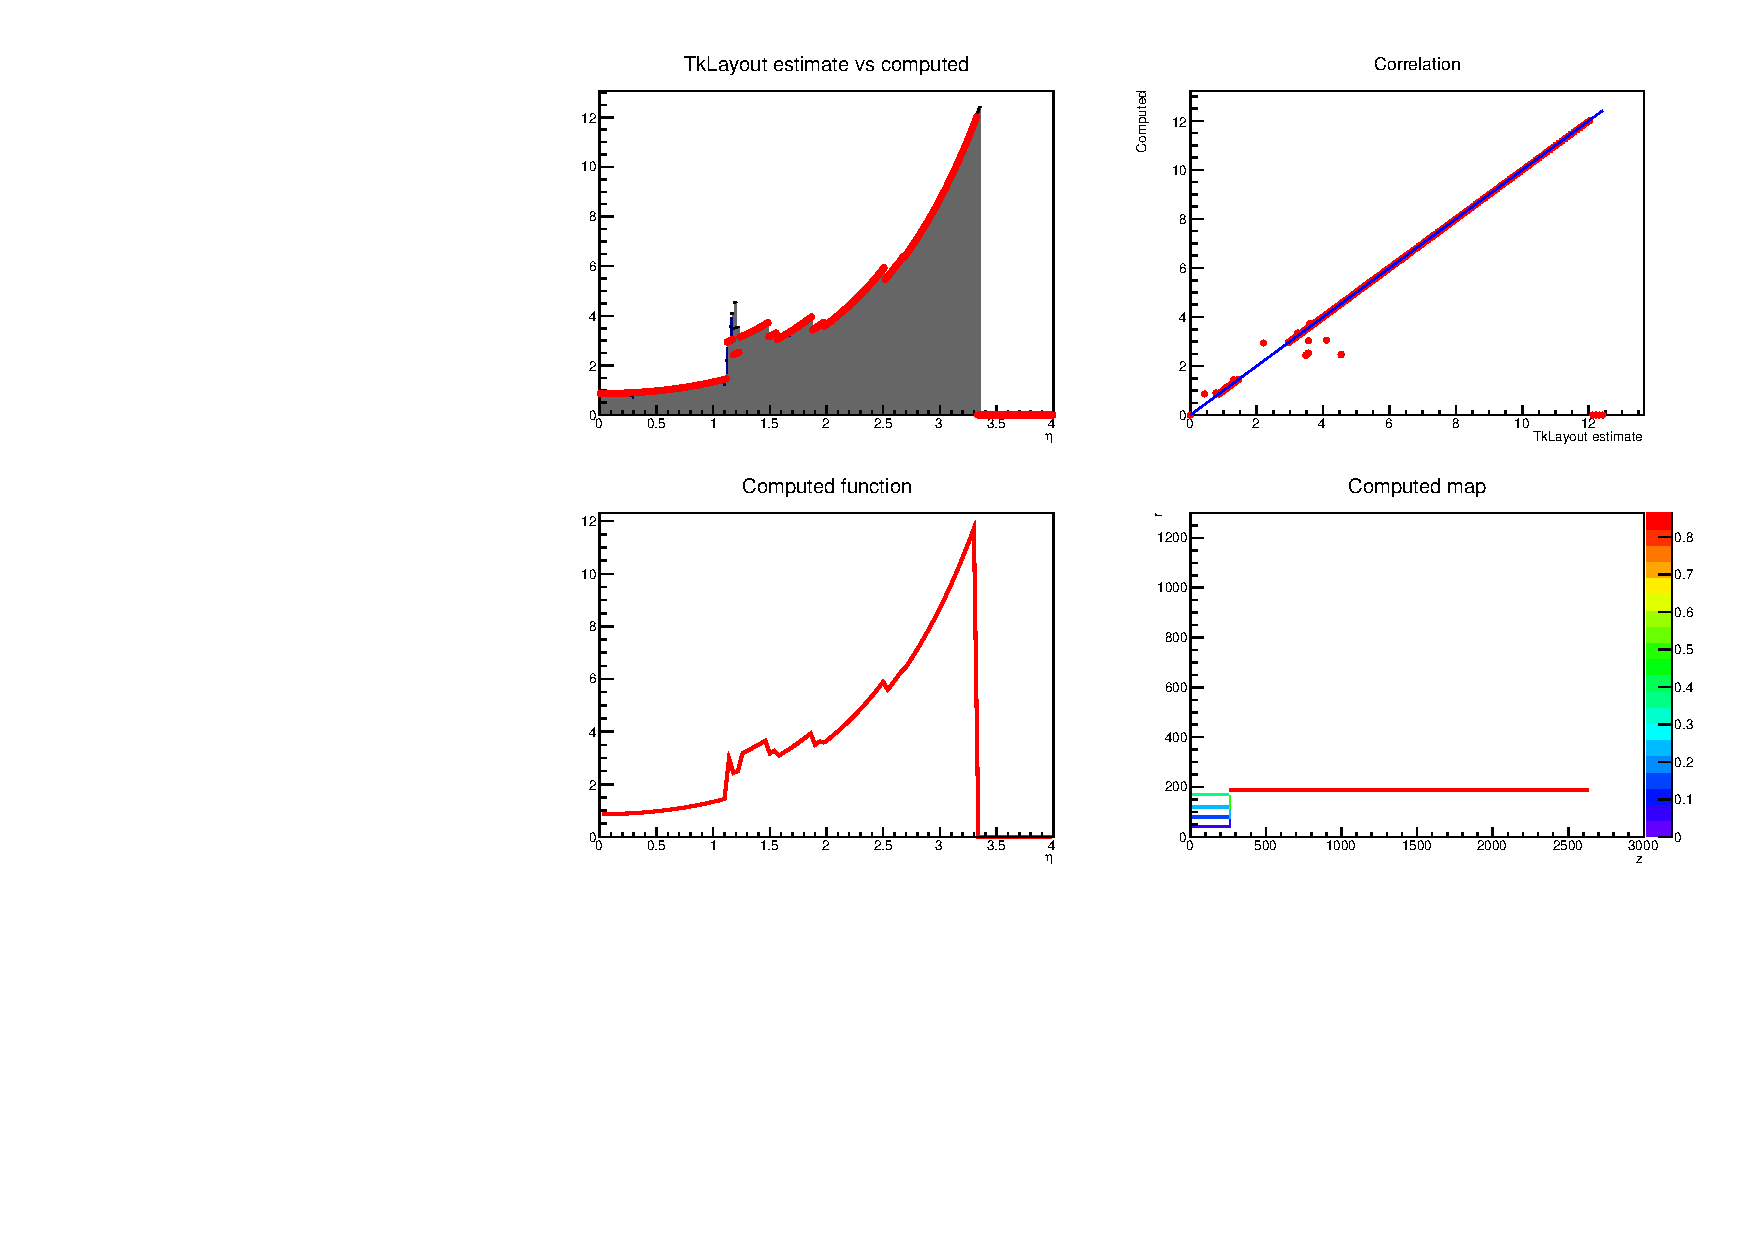
\includegraphics[width=9cm]{img/test3.pdf}
  \end{center}
\end{frame}

\begin{frame}
  \begin{block}{Test4}
    \alert{$100 g/m$} of \emph{Cu} exiting from modules of the first layer of the pixel barrel
    \begin{itemize}
    \item \alert{$L=(rods*100) + L{previous cylinder}$} for cylinders
    \end{itemize}
  \end{block}
  \begin{center}
    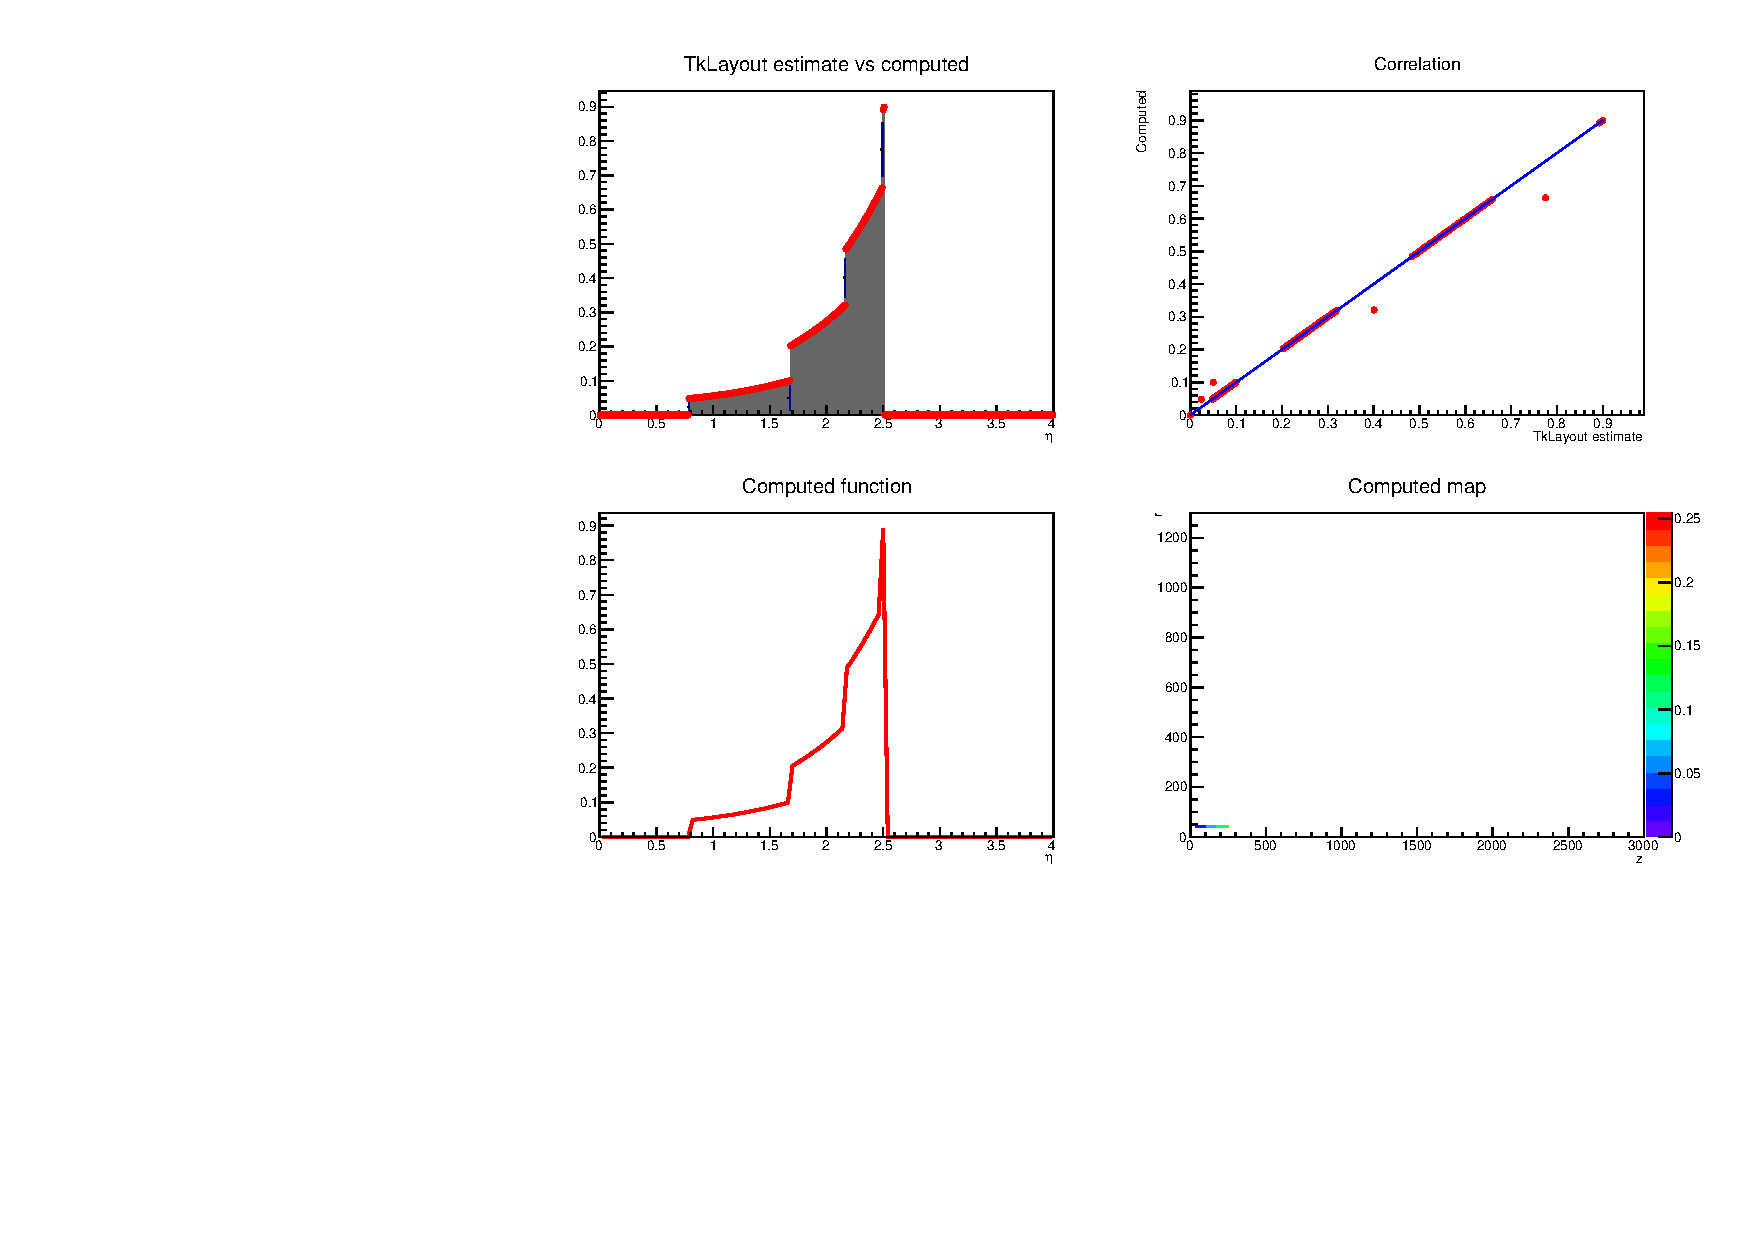
\includegraphics[width=9cm]{img/test4.pdf}
  \end{center}
\end{frame}

\begin{frame}
  \begin{block}{Test5}
    \alert{$100 g/m$} of \emph{Cu} exiting from modules and \alert{$150 g/m$} in the rods
    \begin{itemize}
    \item \alert{$L=(rods*100) + L{previous cylinder}$} for cylinders
    \item \alert{$L=(rods*150)$} in layer
    \end{itemize}
  \end{block}
  \begin{center}
    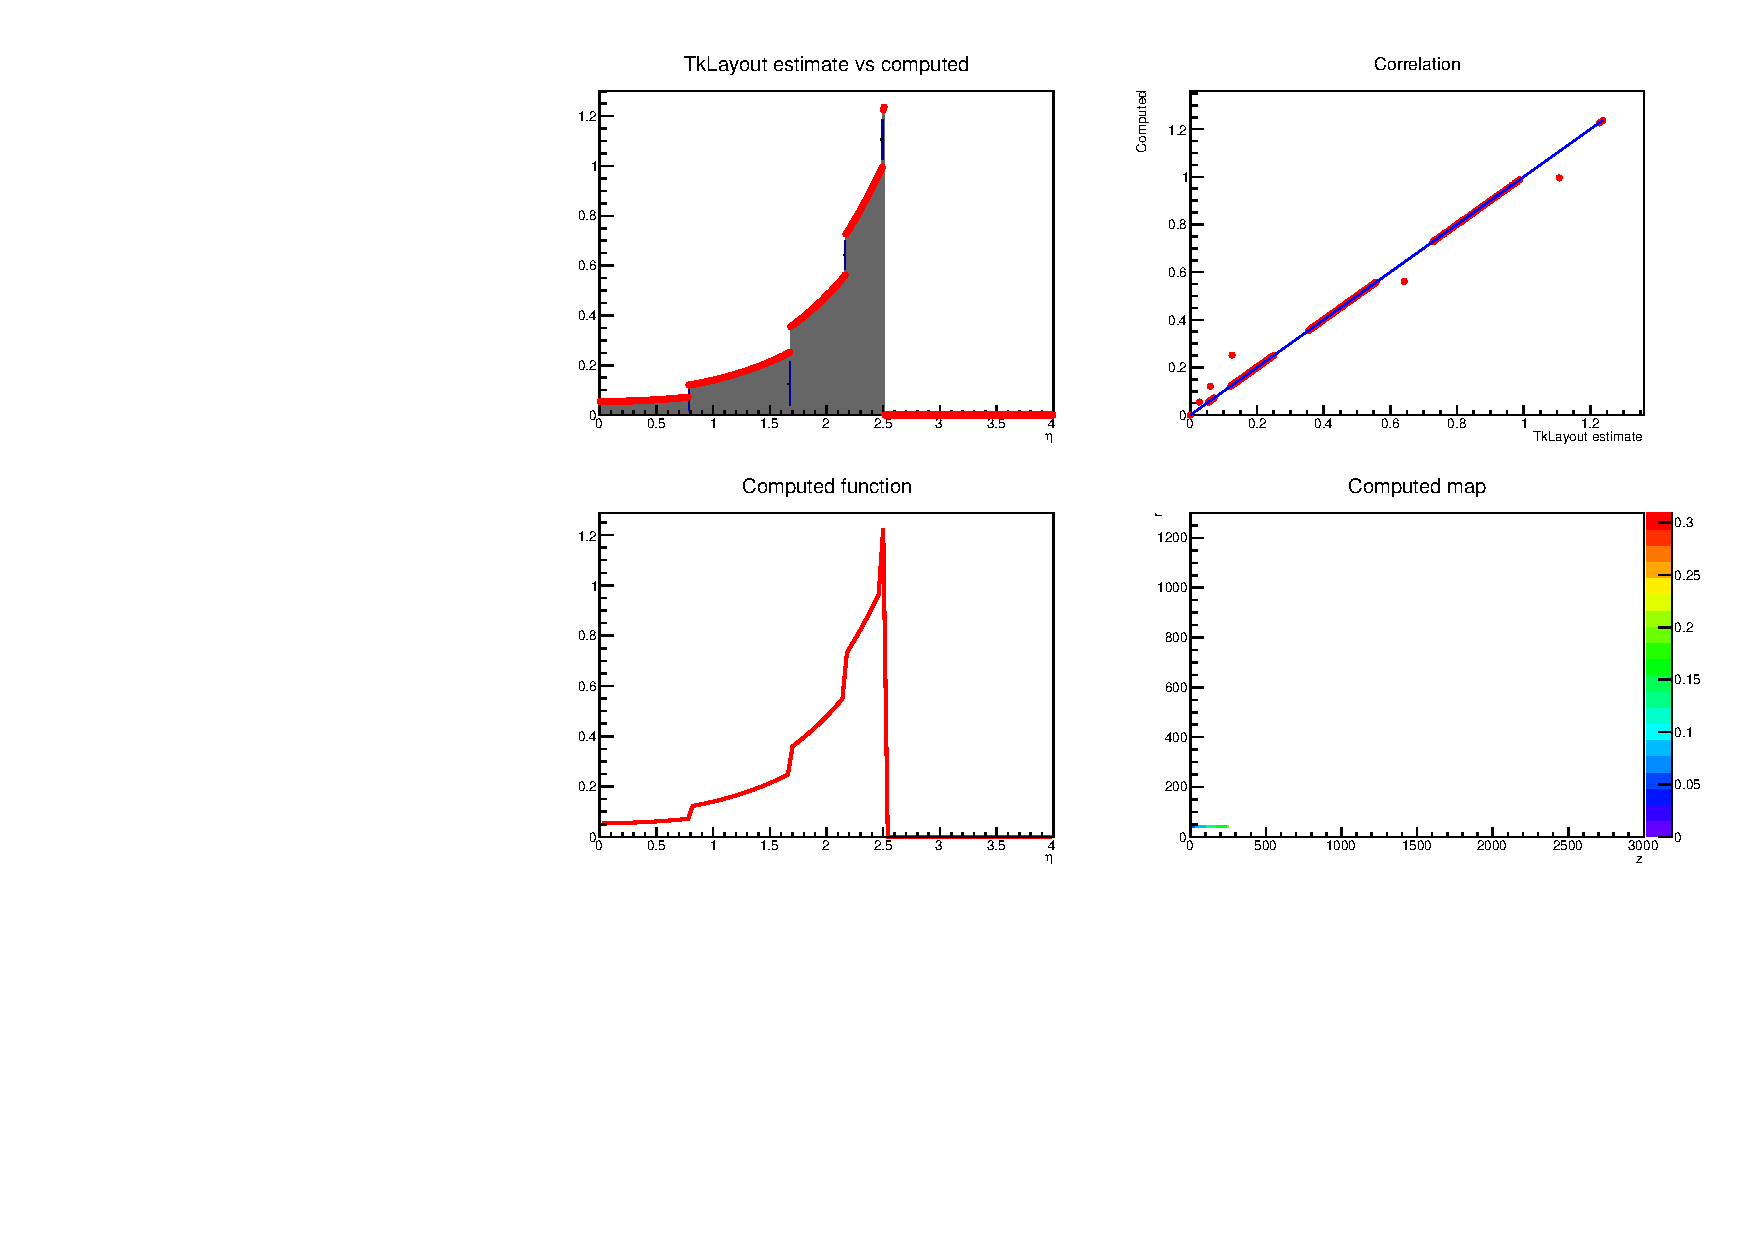
\includegraphics[width=9cm]{img/test5.pdf}
  \end{center}
\end{frame}

\begin{frame}
  \begin{block}{Test6}
    \alert{$100 g/m$} of \emph{Cu} in the first disk of pixel endcap
    \begin{itemize}
    \item \alert{$24$} modules on first ring of disk
    \item \alert{$L=(24*100)$} in every element
    \end{itemize}
  \end{block}
  \begin{center}
    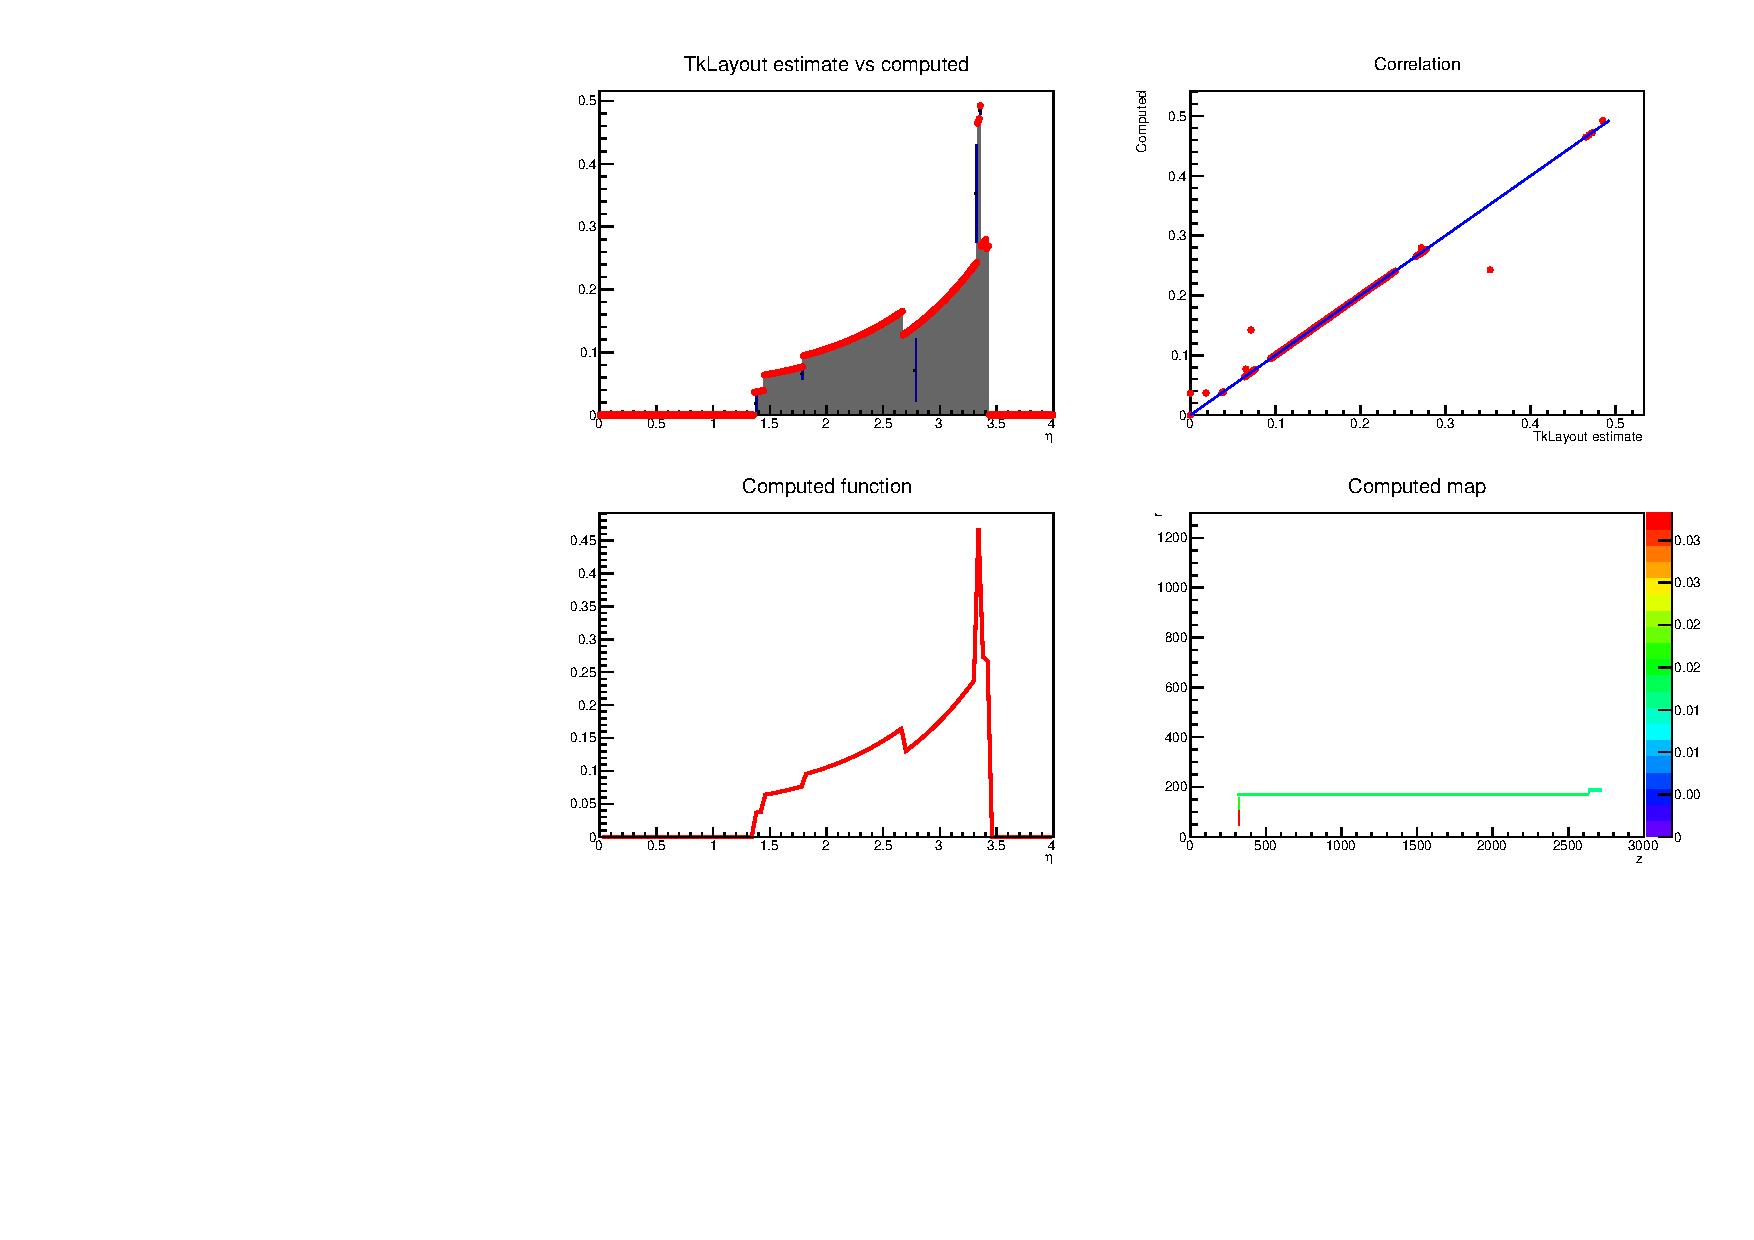
\includegraphics[width=9cm]{img/test6.pdf}
  \end{center}
\end{frame}

\begin{frame}
  \begin{block}{Test7}
    \alert{$100 g/m$} of \emph{Cu} in the fourth layer and conversion \alert{$1g/m\to 0.1g$ locally}
    \begin{itemize}
    \item \alert{$L=(rods*100)$} in layer
    \item \alert{$L=(rods*100*0.1)$} in flange
    \end{itemize}
  \end{block}
  \begin{center}
    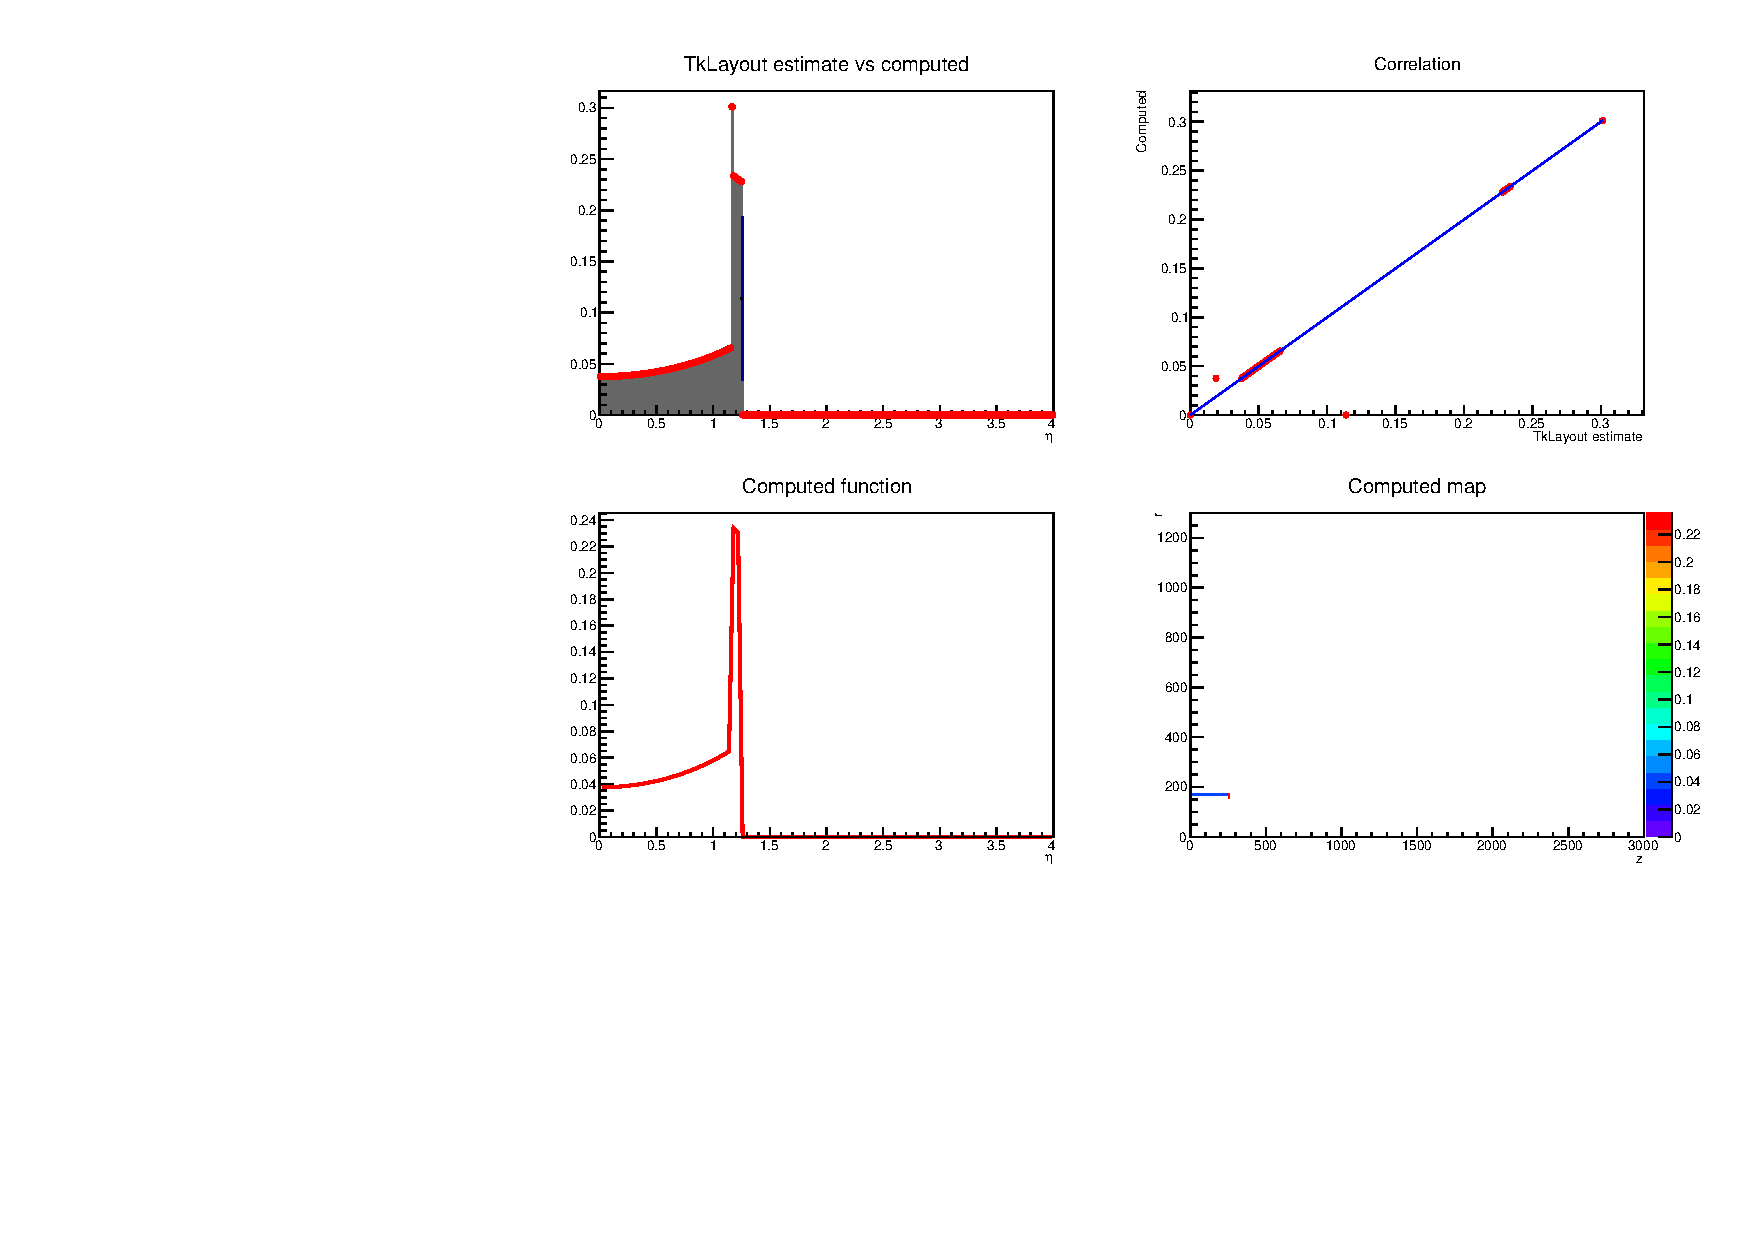
\includegraphics[width=9cm]{img/test7.pdf}
  \end{center}
\end{frame}

\begin{frame}
  \begin{block}{Test8}
    \alert{$100 g/m$} of \emph{Cu} in the fourth layer and conversion \alert{$1g/m\to 1.5g/m$ exiting}
    \begin{itemize}
    \item \alert{$L=(rods*100)$} in layer
    \item \alert{$L=(rods*150)$} in second cylinder
    \end{itemize}
  \end{block}
  \begin{center}
    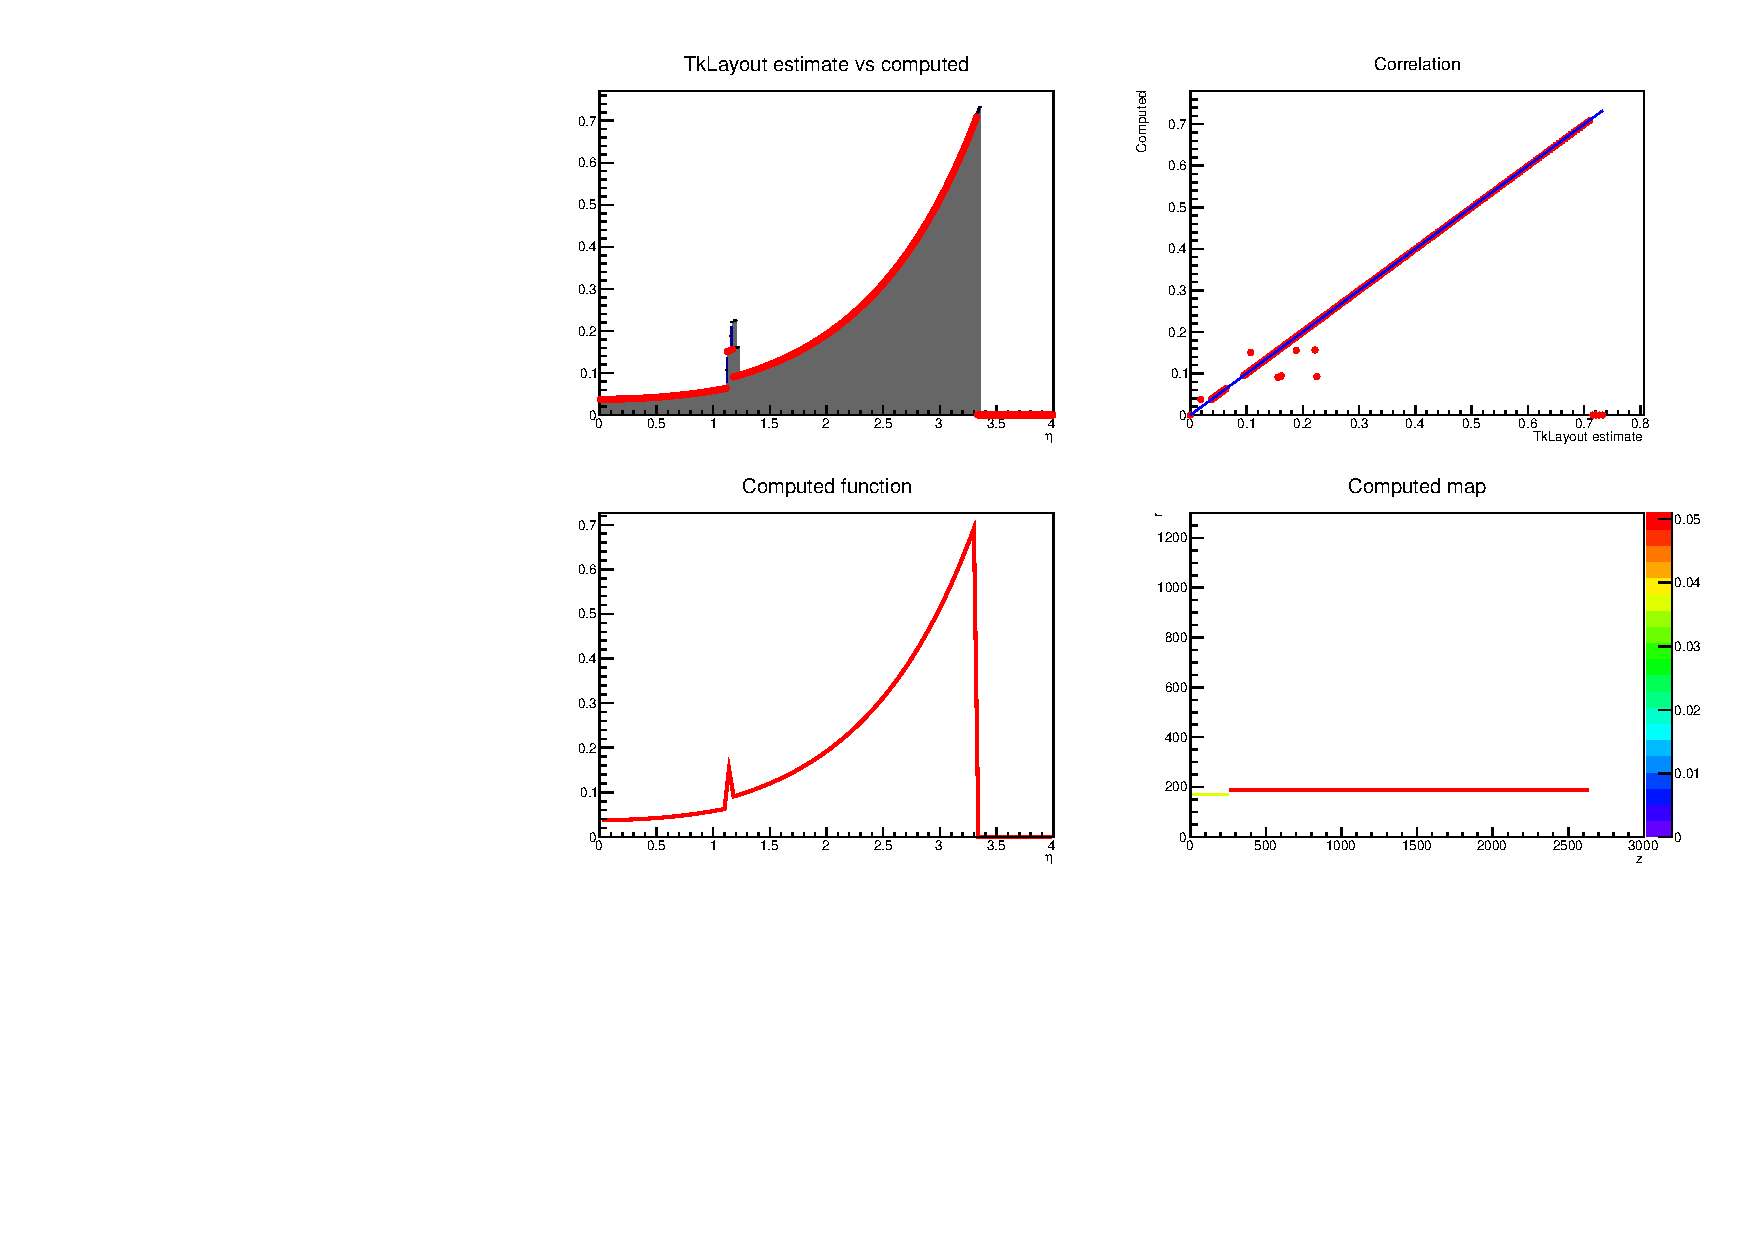
\includegraphics[width=9cm]{img/test8.pdf}
  \end{center}
\end{frame}

\begin{frame}
  \begin{itemize}
  \item Is the testing procedure right?
  \item More kinds of tests?
  \item \alert{Bug} with materials defined in mm
    \begin{itemize}
    \item where replicated for each \alert{rod} in \alert{barrel} and each module of the \alert{first ring} in \alert{endcaps}
    \item[$\to$] corrected but need to be tested
    \end{itemize}
  \item Some supports where defined in \alert{g/m} in endcap
    \begin{itemize}
    \item maybe cause of difference new-old material model?
    \item[$\to$] \alert{corrected} converting them in mm, need to be validated
    \end{itemize}
  \end{itemize}
\end{frame}
\end{document}
